\section{Calibration}
\label{Calibration}

Preliminary energy and timing calibrations of the ECAL were performed in preparation for the CLAS12 engineering
and initial experimental physics runs in 2017-2018. Although the calibration algorithms were already honed from
experience with CLAS, some additional complexity was introduced by the addition of the PCAL and the requirements
of the FPGA-based physics triggers: 

$\bullet$ Differences in the stereo readout geometry of the PCAL imposed the need to incorporate light attenuation
corrections in the trigger firmware to ensure efficiency and spatial uniformity in the cluster energy reconstruction.

$\bullet$ Trigger efficiency studies and overall physics requirements required well-defined cluster energy
thresholds for both electron and MIP triggers in each calorimeter layer (PCAL, ECIN, ECOU).

$\bullet$ Introduction of WLS fibers in the PCAL readout required more accurate time-walk corrections to
compensate for the slower scintillator risetimes in the PMT pulse.

\begin{figure}[hbt]
\centering
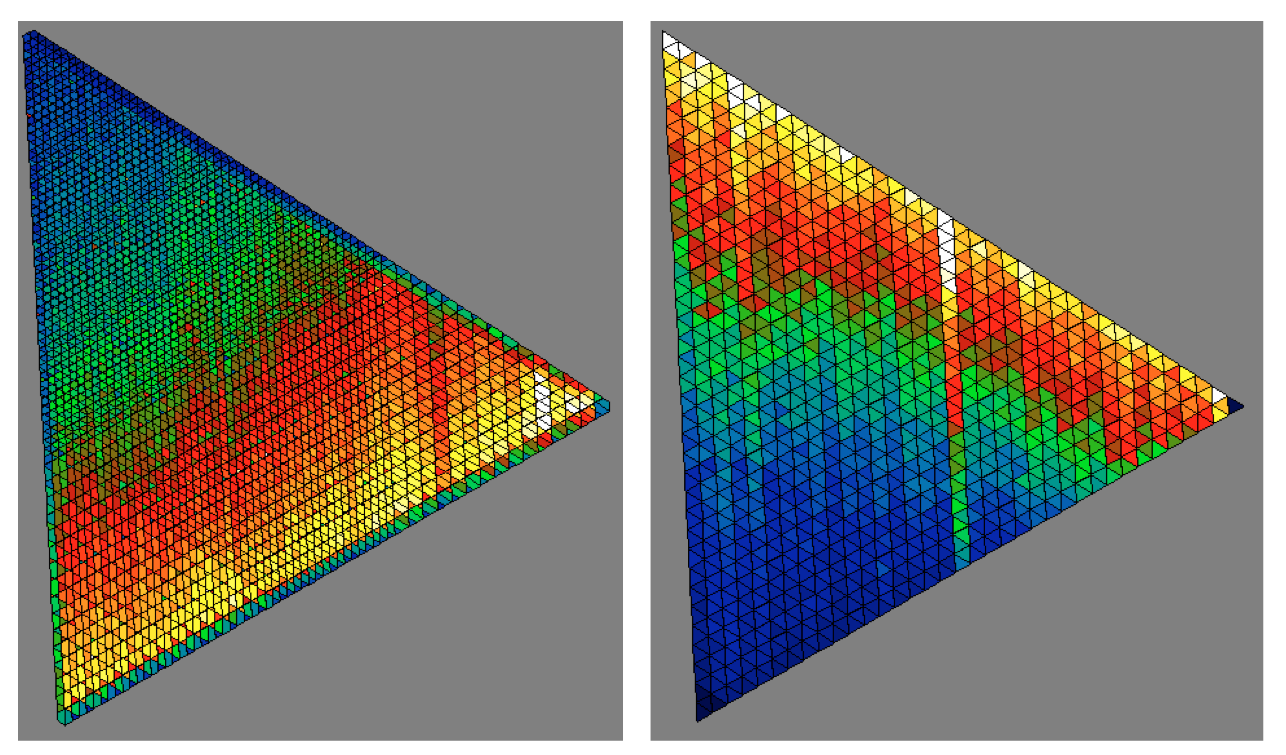
\includegraphics[width=1.0\columnwidth,keepaspectratio]{img/S9_1_1.png}
\caption[]{Pixel map of mean energy loss from MIP muons measured in Sector 5 W PMTs in PCAL (left) and ECIN
  (right). For each map the upper left corner is closest to the beamline. Note in PCAL both V and W strips are readout
  from the base of the triangle, while the ECIN W strips are readout along the right side. The color gradient from
  yellow to blue shows the light attenuation as a function of increasing distance from the readout end of each scintillator.}
\label{fig:S9_1_1}
\end{figure}

\subsection{Energy Calibration}

The longitudinal and transverse segmentation of the ECAL modules together with the requirement for pattern
recognition in the hodoscope design, means that cluster reconstruction from the full detector involves a minimum
of 9 and up to 25 PMTs. The total detected energy $E_{det}$ results from the summation:

\begin{equation}
 E_{det} = \sum_{m}^{3} \sum_{v}^{3} \sum_{n}^{N} E_{n}^{mv},\label{eq:E1}
\end{equation}
\begin{equation}
 E_{n}^{mv} = k(A_{sig}-A_{ped})/(a+c e^{-xb}),   \label{eq:E2}
\end{equation}
\begin{equation}
 E_{tot} = E_{det}/f_{s},                 \label{eq:E3}
\end{equation}
where $E_{n}^{mv}$ is the measured energy in the ${\it n^{th}}$ PMT contributing to the peak in view ${\it v}$ and
module ${\it m}$, and ${\it k}$ is a conversion from FADC units to MeV. The summation occurs over the $N$ PMTs
in each peak, over the 3 U,V,W views for each module, and over the PCAL, ECIN, and ECOU modules. Here the terms $\it{view}$ and $\it{strip}$ always refers to 
the vertical grouping of scintillator strips whose light output is optically summed and measured by a single PMT.  The measured
quantities are ${\it A_{sig}}$, the integrated digitized PMT pulse from the FADC and ${\it A_{ped}}$, the FADC
pedestal. The unknown quantities are the constants $a,b,c$ for the parameterization of the light attenuation as a
function of the distance ${\it x}$ from the cluster to the readout end of the scintillator strip. For EM showers, the
detected energy must be corrected by the sampling fraction $f_{s}$, to obtain the total deposited energy $E_{tot}$.  

Since the energy of an electron incident on the ECAL is known from forward tracking, the energy calibration of the
ECAL is in principle possible by adjusting the $a,b,c$ parameters and the sampling fraction $f_{s}$ until the
reconstructed energy matches the known energy. However, compared to conventional readout geometries, the
relationship in the ECAL between the total deposited energy $E_{tot}$ and the partial energies $E_{n}^{mv}$ is
non-trivial for EM showers. A global optimization would require fitting hundreds of parameters per sector and might
be very slow to converge.

\begin{figure}[hbt]
\centering
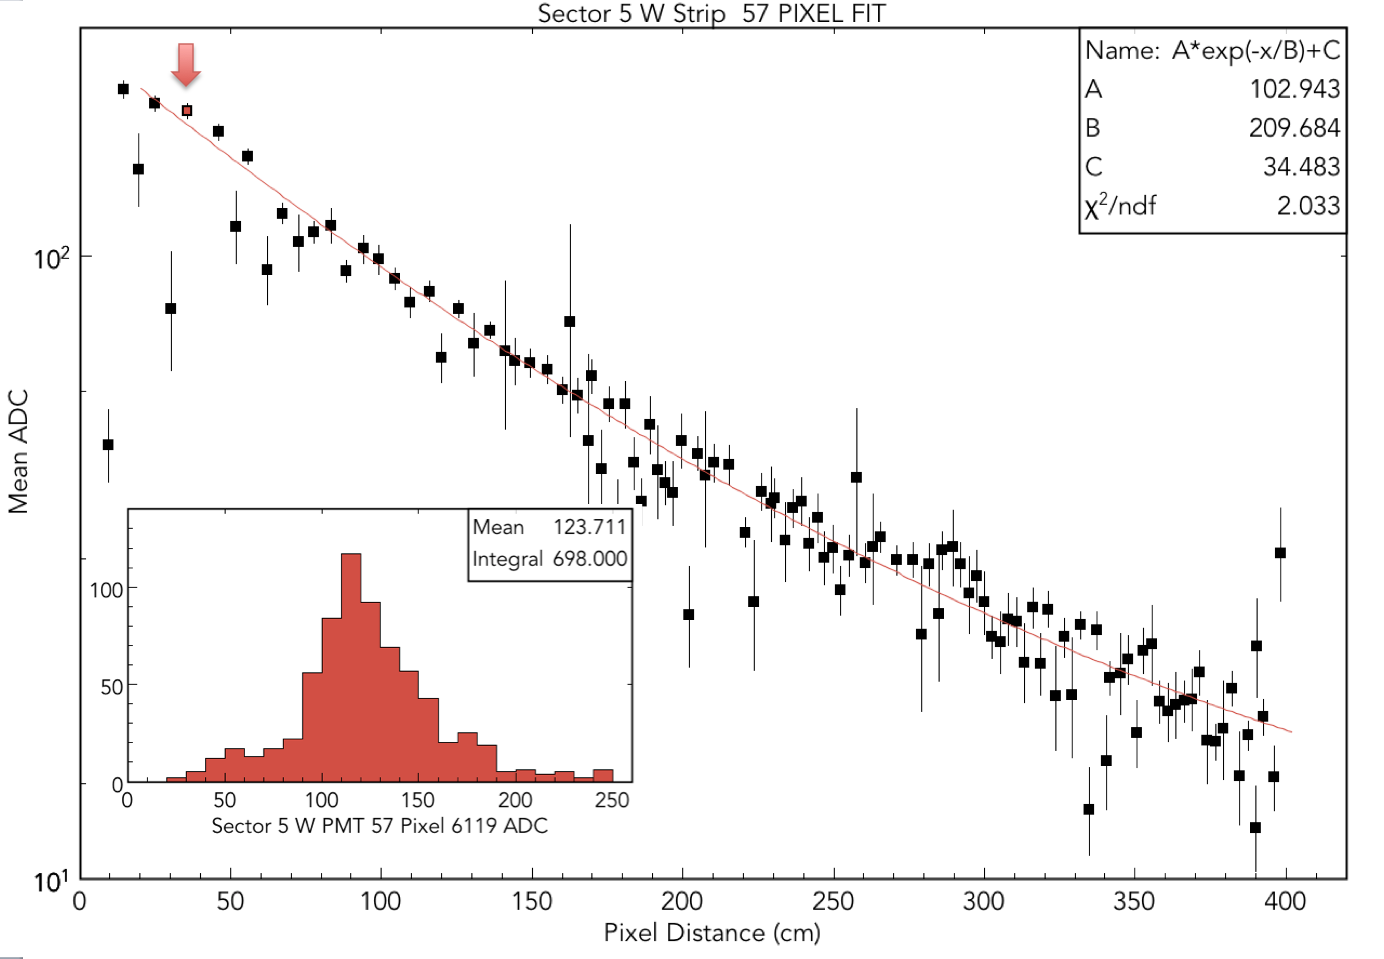
\includegraphics[width=1.0\columnwidth,keepaspectratio]{img/S9_1_2.png}
\caption[]{Typical fits to muon MIP mean energy loss as a function of PCAL pixel distance from the readout end of
  the strip. The inset shows the energy loss distribution in FADC units for the pixel highlighted by the arrow at top.}
\label{fig:S9_1_2}
\end{figure}

A simpler approach used successfully in CLAS with the EC and demonstrated with the PCAL in post-construction testing
described in Section \ref{CRT}, is to proceed iteratively, using minimum-ionizing particles such as cosmic muons to
simplify the energy deposition profile and allow an independent determination of the $a,b,c$ parameters for each
PMT, then adjust the PMT HV to produce a uniform overall response. Later, beam data taken with electrons and
pions is used to estimate ${\it f_s}$ and to cross-check the MIP calibration. With the addition of PCAL to CLAS12
and the introduction of cluster reconstruction in the trigger, pre-calibration with cosmics is critical for evaluating
the trigger performance of the ECAL.

Cosmic runs are performed using a special FPGA trigger that accepts only events where a single pixel has been
activated. A pixel is the simplest possible cluster, and is the smallest unit of $x-y$ position resolution in the ECAL
calorimeters, defined by the overlap of 3 scintillator strips, one from each of the U, V, and W views.  Therefore a pixel must be visualized as a three-dimensional object.  Requiring the
muon to pass through a single pixel places the most restrictive cut possible on the particle track path length,
thereby minimizing the spread in the MIP energy deposition.

A pixel map of the ECAL response to cosmic pixel triggers is shown in Fig.~\ref{fig:S9_1_1} for the W view strips in
the PCAL (left) and ECIN (right). The color gradient in both plots clearly shows the attenuation of light as a function
of readout distance from the pixel, as well as the overall variations in PMT gain near the readout end, such as the
substantially brighter strip in ECIN W19. Also evident is the finer granularity of pixels in the PCAL compared to
ECIN. Note that unlike the ECIN and ECOU modules, which have a constant pixel size, the PCAL pixels have
a variable size and shape due to the mixture of single and double readout strip widths and the different number of
readout strips in U compared to V and W. 

A typical attenuation response plot for a single PCAL PMT (W57) is shown in Fig.~\ref{fig:S9_1_2} from a cosmic
run using a PCAL pixel trigger. The inset shows the energy loss distribution from a single pixel near the readout
end of the scintillator stack and the mean of this distribution for each pixel are the points plotted in the main figure.
The fit shown is used to obtain the ${\it a,b,c}$ calibration constants discussed above. Using this parameterization
the muon MIP peak extrapolated to $x=0$ is ${\it a+c}$. The desired FADC calibration for this peak corresponds
to 10~MeV deposited energy in the 5~cm thick scintillator stack (assuming $dE/dX(MIP)=2$~MeV/cm). PMT high
voltages were iteratively adjusted until the peaks were matched within 5\% of the desired calibration. These gains
were then used for the initial round of data taking with an electron beam.

\begin{figure}[hbt]
\centering
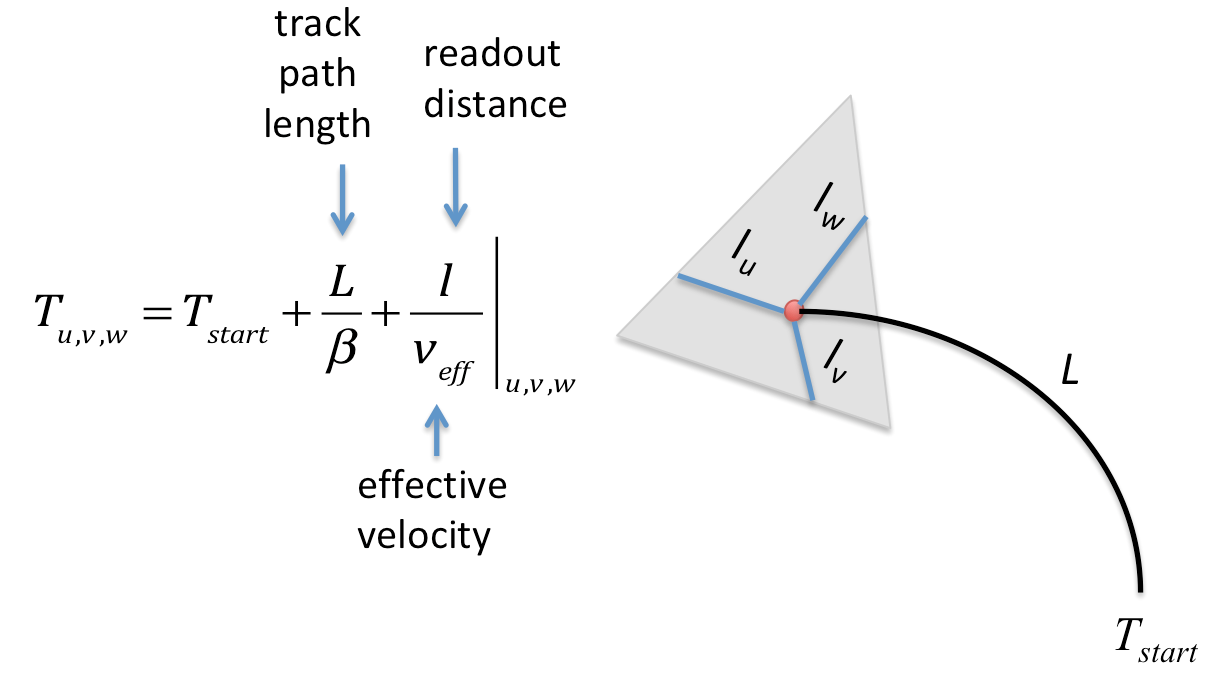
\includegraphics[width=1.0\columnwidth,keepaspectratio]{img/S9_2_0.png}
\caption[]{Cluster readout times $T_{u,v,w}$ at the edges of the calorimeter active area depend on the start time
  $T_{start}$, track path length $L$, and readout distances $l_{u,v,w}$. Particles with velocity $\beta\approx 1$ are
  chosen for calibration, while $v_{eff}$ is extracted from the fits to $T_{measured}$.}
\label{fig:S9_2_0}
\end{figure}

\subsection{Timing Calibration}

Optimal timing calibration in the ECAL is necessary both for neutral particle identification and background rejection.
Identification of neutrons and photons from neutral clusters (those not matched with a charged particle track from
the forward tracking) is based solely on time-of-flight from the target. The stereo readout and modular design of ECAL provides
considerable redundancy in the measurement of cluster timing, due to the multiplicity of PMTs that contribute to the
total cluster energy. This allows flexibility in the choice of PMTs from which to construct the neutral event time. In
addition, this redundancy can be crucial for rejecting accidental clusters formed from randomly overlapping
background hits at high luminosity, especially when attempting reconstruction of neutrons. 

The timing calibration of each PMT is based on analysis of clusters in PCAL, ECIN, and ECOU arising from electrons,
pions, and photons spanning a large range of position and deposited energy. A $\chi^2$ minimization is performed
using six fitted parameters to adjust the difference between the measured time $T_{measured}$ (Eq.~\ref{eq:E4})
and the expected readout time $T_{u,v,w}$ (see Fig.~\ref{fig:S9_2_0}). These are defined, respectively, as:

\begin{equation}
T_{measured}=t_{TDC}+t_{ADC} \label{eq:E4}
\end{equation}
\begin{equation}
t_{TDC}=a_0+a_1\times~TDC \label{eq:E5}
\end{equation}
\begin{equation}
t_{ADC}=\frac{a_2+300(100)}{ADC^{1/2}}+a_3+\frac{a_4}{ADC^{1/4}} \label{eq:E6}
\end{equation}
where the free parameters are the five "a" coefficients and the light effective velocity $v_{eff}$.

Unit conversion of the raw TDC measurements and determination of cable delays are absorbed into the $t_{TDC}$ term (Eq.~\ref{eq:E5}). Corrections due to the
amplitude dependence of the discriminated PMT pulse time are parameterized in $t_{ADC}$ (Eq.~\ref{eq:E6}) using
the integrated pulse from the FADC.  Finally, the scintillator effective velocity $v_{eff}$ parameterized in $T_{u,v,w}$
is extracted from fits to $T_{measured}$. The $t_{TDC}$ and $t_{ADC}$ fits are performed alternately and iterated
until convergence is reached. The $t_{TDC}$ fits are initialized with $a_2$, $a_3$ and $a_4$ in $t_{ADC}$ set to zero,
using a fixed correction of 300(100) for PCAL(EC).

The procedure requires knowledge of the event start time $T_{start}$, the path length $L$ from the target vertex
to the cluster position, together with the readout distances $l_{u,v,w}$ from the cluster as indicated in
Fig.~\ref{fig:S9_2_0}. These quantities are supplied by the various reconstruction services. Note that $T_{start}$
is synchronized to the RF pulse containing the incident electron and also compensates for the extended target
vertex position.

For calibration purposes the cluster time is defined by the single PMT having the largest ADC value, in order to
minimize the time-slew correction and maximize photon statistics. Typical uncertainties in the calibrated cluster
time residuals are shown in Fig.~\ref{fig:S9_2_1} for the PCAL and ECIN U PMTs in Sector~1. The points show the
means of Gaussian fits to the residual distributions from each strip, where the mean variance is within 50~ps. The
vertical red lines show the $\sigma$ of the fits, which represents the timing resolution averaged over all peak
energies visible to that strip.  

\begin{figure}[hbt]
\centering
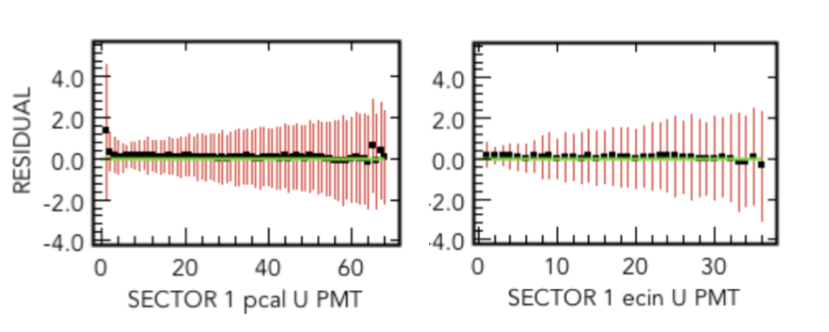
\includegraphics[width=1.0\columnwidth,keepaspectratio]{img/S9_2_1.png}
\caption[]{Residuals ($T_{measured}-T_{u,v,w}$) of calibrated cluster times in nanoseconds, plotted versus U strip
  PMT numbers in the PCAL (left) and ECIN (right) calorimeters. The vertical red lines indicate the $\sigma$ of
  Gaussian fits to the residual distributions.}  
\label{fig:S9_2_1}
\end{figure}

The deposited energy dependence of the timing resolution for typical strips in PCAL and ECIN is shown in
Fig.~\ref{fig:S9_2_2}, which clearly shows the improvement in resolution with increasing photon statistics. Although
the PCAL has a 3-4 times larger light yield compared to the EC, the broader time distribution of photons due to the
WLS fiber conversion of the bulk scintillator light results in a somewhat worse resolution compared to the EC. Future
development of the timing reconstruction will utilize both TDC and FADC derived timing from multiple PCAL and EC
PMTs to determine the optimal contribution needed to provide the most accurate total energy cluster time.

\begin{figure}[hbt]
\centering
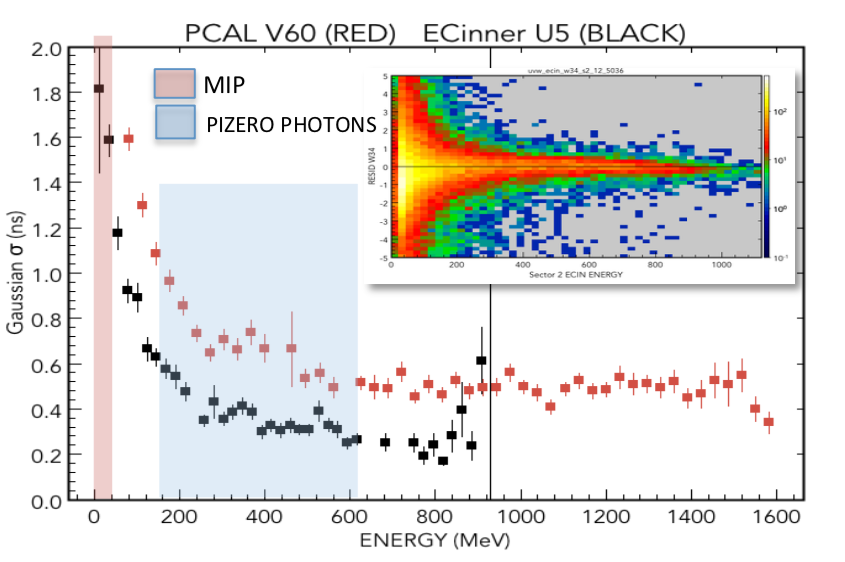
\includegraphics[width=1.0\columnwidth,keepaspectratio]{img/S9_2_2.png}
\caption[]{Deposited energy dependence of the timing resolution for typical strips in PCAL and ECIN. The red
  and blue bands show the energy ranges dominated by MIP pions and photons associated with
  $\pi^0\rightarrow 2\gamma$ decays, respectively. The inset shows the 2D distribution of residual vs. energy
  for PCAL.}
\label{fig:S9_2_2}
\end{figure}


